% =====================================================================================================
% Appendix: experimental details (A), additional results (B), analysis of probe relocation (C),
% example maps (D) and key code (E). Parameter-randomisation results are included in B.
% =====================================================================================================

\counterwithin{figure}{section}
\counterwithin{table}{section}
\captionsetup{skip=5pt}
\raggedbottom

\section{Experimental details}
\label{app:setup}

\paragraph{Models.} All models are frozen ViTs with $16{\times}16$ patches on $224{\times}224$ inputs, taken from timm~\citep{wightman2019}. \emph{DeiT-S and DeiT-B}~\citep{touvron2021}: \texttt{deit\_small\_patch16\_224.fb\_in1k} and \texttt{deit\_base\_patch16\_224.fb\_in1k} (resize to 248, centre crop 224: a crop ratio of 0.9). \emph{DINO ViT-S/16}~\citep{caron2021}: \texttt{vit\_small\_patch16\_224.dino} with the official DINO linear head (resize to 256, centre crop 224: a crop ratio of 0.875). \emph{DeiT-S with a test-time register}~\citep{jiang2025}: the activations of eight feed-forward units in layers 4 and 5 are moved to one added register token, which is left out of every map, like CLS. The units were selected on 500 ImageNet-S images, where they reduce the number of high-norm patch tokens (counted per layer) by 92.75\% and keep 99.0\% of the predictions; on the other 11,919 images the reduction is 91.5\%, and ImageNet accuracy stays at 79.8\%. For DeiT-B the same search found no such units (44.9\% reduction with 32 units), so we report the register for DeiT-S only. \emph{Top-$k$ training}: the DeiT-S checkpoint released with MiTA~\citep{wen2026mita} (25 summary slots, $k=25$), with its own preprocessing (crop ratio 0.875). It differs from our DeiT-S in training and preprocessing, so its row in Table~\ref{tab:main} is not a controlled comparison; its deletion score is undefined because its summary slots pool fixed regions of the full grid. Both model-side fixes are tested at size S only; in a preliminary comparison with an earlier protocol, top-$k$ training scored 0.011 lower in object enrichment than its baseline at size S but 0.037 higher at size Tiny, so the result should not be read beyond DeiT-S.

\paragraph{Attention conventions.} With $x$ the block input after its first layer norm, projections include the checkpoint's biases:
\[
q_i^h=W_Q^hx_i+b_Q^h,\quad k_j^h=W_K^hx_j+b_K^h,\quad v_j^h=W_V^hx_j+b_V^h.
\]
Equation~\ref{eq:attn} includes the output bias $b_O$ and describes the attention branch before residual addition, with dropout inactive at evaluation. $W_O^h$ is the head's slice of the output projection. C3 assigns the per-head vector magnitudes to patches; the shared output bias is not assigned to any patch. The fixed-image two-layer representation uses the coupled softmax activation, rather than an elementwise nonlinearity.

\paragraph{Data.} \emph{Execution test}: 5,000 randomly drawn ImageNet validation images~\citep{deng2009}. \emph{ImageNet-S}~\citep{gao2023}: all 12,419 validation images with segmentation masks; enrichment is defined for 12,150 (12,144 for DINO) after excluding images without valid foreground or background patches. Deletion uses a fixed random subset of 2,000. \emph{ClickMe}~\citep{linsley2019,fel2022}: the 17,408-image validation split released with Harmonization (17 \texttt{val-*.tfrecords} shards). This split name does not identify the original ImageNet split of each image. Images are resized from $256{\times}256$ to $224{\times}224$ without cropping; heatmaps are resized to $64{\times}64$, blurred with a $10{\times}10$ Gaussian ($\sigma=10$), then resized to $224{\times}224$ (bilinear interpolation). \emph{Held-out set}: 4,000 ImageNet validation images excluded from map-quality and execution evaluation; 2,000 train probes and 2,000 provide mean maps, probe-test accuracies and blur calibration. Our near-duplicate check matched 2 of 4,002 candidate ImageNet validation images to ClickMe records; this does not establish every ClickMe image's training-set membership. Possible overlap with model training images limits generalisation claims.

\paragraph{Diagnostics.} All three are computed per layer. \emph{Specificity}: with $\bar s$ the mean received-attention map of the held-out images and $\operatorname{Var}_j$ the variance over the 196 patches of one image, the share explained is $1-\sum_x\operatorname{Var}_j(s-\bar s)\,/\sum_x\operatorname{Var}_j(s)$, summed over the ImageNet-S images $x$. \emph{Location}: the top-1 accuracy of the linear position probe on the 196 patch tokens of each of 2,000 held-out images. \emph{Contribution}: the share of received attention on high-norm tokens, on the ImageNet-S images. The high-norm threshold (three times the median, defined below) is an operational definition fixed before the experiments; we did not test other thresholds. The correction itself uses no threshold.

\paragraph{Corrections and matched controls.} Scores are computed per layer and summed over layers 9--12 without per-layer rescaling, except for the C1 control's calibration described below. Queries include all 197 tokens; maps contain 196 patches. Negative C1 scores are retained for ranking, without clipping.
\emph{Mean-map subtraction} computes $\sum_\ell(s_\ell-\bar s_\ell)$ using the 2,000 calibration images. With $S=\sum_\ell s_\ell$ and $\bar S=\sum_\ell\bar s_\ell$, its control is $S-G\,\operatorname{sd}_j(\bar S)/\operatorname{sd}_j(G)$, where $G$ is a centred isotropic Gaussian ($\sigma=3.5$ patches). Calibration thus uses the \emph{summed} mean map.
\emph{Probe relocation} computes $r_p=\sum_j s_jP_\ell(p\mid x_j)$, preserving total score. One linear 196-way classifier per model/layer is trained on standardised tokens after the first layer norm: cross-entropy, Adam, learning rate 0.01, 30 epochs, token minibatches of 4,096, seed 0. Feature means/standard deviations use only the 2,000 training images; standard deviations are floored at $10^{-6}$. Its Gaussian control is a row-normalised kernel $K_{jp}\propto\exp(-\lVert p-j\rVert^2/(2\sigma_\ell^2))$. The width (0.7--2.9 patches) matches
\[
D_\ell=\frac{1}{2000N}\sum_{x,j,p}P_\ell(p\mid x_j)\lVert p-j\rVert^2
\]
on calibration images, using uniform averaging over source patch indices. It does not match attention-weighted score-mass displacement.
\emph{Contribution weighting} computes $c_j=\sum_{h,i}a_{ij}^h\lVert W_O^hv_j^h\rVert_2$, a sum of per-head norm-weighted terms related to \citet{kobayashi2020}. Summing magnitudes before aggregating across heads omits cross-head cancellation; residual addition, subsequent normalisation and later-layer computation are outside this score. The control zeros received attention at high-norm patches: block-input norm greater than three times the image's median patch norm, using the midpoint median. C3 itself has no high-norm threshold.
\emph{All three corrections}: contribution weighting, probe relocation, then subtraction of the held-out mean of the resulting map, per layer before summation.

\paragraph{Metrics.} \emph{Same-ring object enrichment.} A patch is valid if it contains at least one non-ignored pixel, and is an object patch if at least half of its non-ignored pixels belong to the image's class mask. We select as many top-scoring patches as there are object patches. For every ring of patches at the same distance from the grid centre, we take the object rate among its selected patches minus that among all its patches, and average over rings, weighted by their selected patches. Invalid patches are excluded from selection and ring baselines. Ties are broken with the fixed seeded perturbation used in the original runs. A purely radial map scores zero in expectation over tie-breaking.
\emph{Image-specific ClickMe alignment.} The map is upsampled to $224{\times}224$ and correlated (Spearman, over pixels) with the image's own human map; we subtract its correlation with the previous image's human map within each batch (\texttt{roll(1)}; batch size 64). For an image-independent map, these differences average to zero over the paired set because the control permutes the same human maps; individual-image differences need not be zero. This removes fixed-prior alignment on average, without guaranteeing invariance to a prior mixed into an image-dependent map.
\emph{Deletion score.} Patches are ranked once by the original map. At removal budgets $0,1,2,4,8,16,32,64,98,147$, we record the binary indicator that the original top-1 prediction is preserved. Tokens are dropped after positional embedding; CLS and any register remain. We use an SRG-style LIF--MIF area difference~\citep{bluecher2024}, adapting the value function from class probability to top-1 preservation. Areas use trapezoidal integration over removed-patch fraction $b/196$, from 0 to $147/196$.
\emph{Validity of the metrics.} A random map, a centred Gaussian and the mean map all score within 0.004 of zero on enrichment and on ClickMe alignment (the two image-independent maps have exactly zero mean on the latter, up to numerical precision); on deletion the centred Gaussian scores 0.110, 0.099 and 0.140 (DeiT-S, DeiT-B, DINO ViT-S), which is why every correction is compared with a matched control.
\emph{Statistics.} One value per image; paired image-bootstrap with 1,000 resamples, seed 0 and 95\% percentile intervals. A difference is \emph{higher} (\textit{h}) or \emph{lower} (\textit{l}) if its interval excludes zero and its absolute mean reaches 0.02 (0.05 for deletion), and \emph{comparable} (\textit{c}) otherwise. These unchanged registered categories do not establish equivalence. Intervals are unadjusted for multiple comparisons. Resampling holds checkpoints, probes and the within-batch ClickMe pairing fixed, excluding uncertainty from training, probe fitting or alternative pairings. Because the control reuses human maps within each batch, ClickMe score rows are not independent pairings.

\paragraph{GAE reference.} The gradient-based reference~\citep{chefer2021generic} targets the unmodified model's predicted top-1 logit and uses all 12 attention layers. Starting with $R=I$, each layer updates $R\leftarrow R+\operatorname{mean}_h[(\nabla_{A^h}f_c\odot A^h)_+]R$, then takes the final CLS-to-patch row. It is class-specific and spans all layers, whereas R0/C1--C3 are class-agnostic and sum layers 9--12. Its scores provide descriptive context rather than a matched single-component ablation.

\paragraph{Registered predictions.} The protocol was frozen before formal runs, after smoke tests on 32--64 images and earlier exploratory observations documented in \texttt{docs/preregistration.md}. Historical P4/P3/P6 map to R1/R2/R3; definitions, margins and verdicts are unchanged. R2 has three possible outcomes: holds (4/4 higher), partly holds (1--3) and does not hold (0). Primary contrasts were the combination versus R0 and each correction versus its matched control, without a registered direction for the latter. Other correction--R0 contrasts are descriptive, except R1's registered negative controls. Prior execution/diagnostic results had been seen, making the last two rows of Table~\ref{tab:app-registered} replications. Diagnosis--benefit interpretation and supplementary mechanism analyses are post hoc.

\begin{table}[!htbp]
\caption{Registered predictions and outcomes (centre-controlled metrics: enrichment and ClickMe alignment).}
\label{tab:app-registered}
\centering\footnotesize
\setlength{\tabcolsep}{4pt}
\begin{tabular}{@{}l>{\raggedright\arraybackslash}p{3.55in}>{\raggedright\arraybackslash}p{1.35in}@{}}
\toprule
 & Prediction & Outcome\\
\midrule
R1 & Contribution weighting is comparable to received attention in DINO ViT-S on all three metrics & holds (3 of 3 cells)\\
R1 & Relocation at layers 1--4 is comparable to received attention on the centre-controlled metrics in all models & holds (6 of 6 cells)\\
R2 & All three corrections together are higher than received attention on the centre-controlled metrics in DeiT-S and DeiT-B & partly holds (1 higher: DeiT-B ClickMe; 1 comparable; 2 lower)\\
R3 & Neither model-side change is higher than DeiT-S received attention on the centre-controlled metrics & holds (4 of 4 cells)\\
\midrule
-- & Execution agreement rises with $k$ and exceeds that of random sets at every $k$ & holds in all models\\
-- & Probe accuracy falls with depth; the share of attention on high-norm tokens peaks in layers 6--12 of the supervised models and is below 1\% in every layer of DINO ViT-S & holds in all models\\
\bottomrule
\end{tabular}
\end{table}

\paragraph{Compute and code.} Experiments took about 19 NVIDIA L4 GPU hours. Code, configurations, fixed splits, checkpoint revisions and recorded provenance: \url{https://github.com/hhuang999/vit-fastweight-lens}. The release supplies \texttt{configs/}, \texttt{data/splits/} and \texttt{docs/provenance/}; unavailable historical environment fields remain unknown. Presentation changes use stored evidence, without rerunning experiments.

% =====================================================================================================
\section{Additional results}
\label{app:more}

These results support the framework at different levels: execution and parameter sensitivity check internal dependence, while paired comparisons and supplementary analyses assess map quality and proposed interpretations.
\suppressfloats[t]

\paragraph{Execution test.} The $14{\times}14$ grid is pooled into 16 overlapping regions. In every layer/head, each region's mean query selects its top-$k$ keys; CLS retains its own set. Sets from an unmodified forward pass restrict every query to its region's set in all 12 layers simultaneously. Top-$k$ sets beat equal-size random sets at every tested $k$ (4--128) in all models, and agreement rises with $k$ (Fig.~\ref{fig:app-ksweep}). The dotted attention-removed baseline alone uses uniform crop ratio 0.875; solid/dashed DeiT curves use 0.9.

\begin{center}\begin{minipage}{3.6in}
\centering
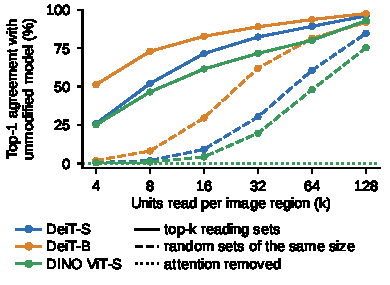
\includegraphics[width=3.25in]{execution_k_sweep}
\captionof{figure}{Top-1 agreement on 5,000 ImageNet images with region-selected top-$k$ units (solid), random units (dashed) or attention removed (dotted). Stored 95\% intervals are at most $\pm1.5$ percentage points. Dotted curves use crop ratio 0.875 for all models; other curves use each checkpoint's main preprocessing.}
\label{fig:app-ksweep}
\end{minipage}\end{center}

\paragraph{Diagnostics per layer.} Table~\ref{tab:app-diag} lists the diagnostics plotted in Fig.~\ref{fig:diag}a--c and the uncorrected per-layer ClickMe alignment. Two further details complement the table. First, in layers 9--12, 82--98\% of the variance of the mean map is explained by the distance from the grid centre. Second, averaged over layers 9--12, the mean value-vector norm $\lVert v_j\rVert$ of high-norm tokens is 0.29 (DeiT-S) and 0.23 (DeiT-B) times the median of the other patches (measured on 11,919 ImageNet-S images using uniform crop ratio 0.875, unlike the main DeiT evaluation at 0.9).

\paragraph{Recovery at the last layer.} In the supervised models, single-layer received attention is worse at layer 12 than at the best of layers 8--11 (ClickMe values in Table~\ref{tab:app-diag}). Applied to layer 12, contribution weighting recovers 62\% and 33\% of this drop on enrichment (DeiT-S, DeiT-B), 31\% and 45\% on ClickMe alignment, and 8\% and 29\% on deletion. The other two corrections make layer 12 worse.

\begin{table}[!htbp]
\caption{Per-layer diagnostics (Fig.~\ref{fig:diag}a--c) and uncorrected ClickMe alignment (last three columns). S, B, D: DeiT-S, DeiT-B, DINO ViT-S; probe chance: 0.5\%. Values are rounded; DINO layers 9--12 have exactly zero high-norm attention on this dataset.}
\label{tab:app-diag}
\centering
% Per-layer diagnostics, generated from results/diagnose.csv by diag_table.py.
\footnotesize
\setlength{\tabcolsep}{2.6pt}
\begin{tabular}{r >{\centering\arraybackslash}p{0.8cm} >{\centering\arraybackslash}p{0.8cm} >{\centering\arraybackslash}p{0.8cm} >{\centering\arraybackslash}p{0.8cm} >{\centering\arraybackslash}p{0.8cm} >{\centering\arraybackslash}p{0.8cm} >{\centering\arraybackslash}p{0.8cm} >{\centering\arraybackslash}p{0.8cm} >{\centering\arraybackslash}p{0.8cm} >{\centering\arraybackslash}p{1.05cm} >{\centering\arraybackslash}p{1.05cm} >{\centering\arraybackslash}p{1.05cm}}
\toprule
 & \multicolumn{3}{c}{\makecell{Specificity:\\mean-map share (\%)}} & \multicolumn{3}{c}{\makecell{Location:\\probe accuracy (\%)}} & \multicolumn{3}{c}{\makecell{Contribution:\\high-norm share (\%)}} & \multicolumn{3}{c}{\makecell{Map quality:\\ClickMe alignment}} \\
\cmidrule(lr){2-4}\cmidrule(lr){5-7}\cmidrule(lr){8-10}\cmidrule(lr){11-13}
Layer & S & B & D & S & B & D & S & B & D & S & B & D \\
\midrule
1 & 6.8 & 12.4 & 11.2 & 100.0 & 100.0 & 99.9 & 0.0 & 0.0 & 0.0 & $-$0.108 & $-$0.111 & $-$0.089 \\
2 & 21.2 & 14.0 & 7.4 & 100.0 & 100.0 & 100.0 & 0.0 & 0.0 & 0.0 & 0.007 & 0.041 & 0.064 \\
3 & 13.7 & 15.0 & 19.7 & 99.9 & 100.0 & 99.9 & 0.0 & 0.0 & 0.0 & 0.081 & 0.004 & 0.056 \\
4 & 6.9 & 7.5 & 14.6 & 99.0 & 100.0 & 99.8 & 0.0 & 0.0 & 0.0 & 0.132 & 0.110 & 0.140 \\
5 & 7.8 & 5.8 & 14.6 & 97.5 & 99.9 & 99.6 & 0.1 & 0.0 & 0.0 & 0.148 & 0.130 & 0.150 \\
6 & 5.2 & 6.2 & 11.9 & 85.3 & 99.5 & 98.9 & 2.6 & 0.0 & 0.0 & 0.136 & 0.151 & 0.167 \\
7 & 4.4 & 5.4 & 12.4 & 65.0 & 96.8 & 95.9 & 7.4 & 3.5 & 0.0 & 0.147 & 0.131 & 0.150 \\
8 & 4.2 & 5.4 & 6.6 & 43.9 & 91.8 & 85.6 & 9.3 & 12.9 & 0.0 & 0.149 & 0.118 & 0.170 \\
9 & 4.2 & 5.7 & 9.5 & 31.0 & 83.6 & 67.4 & 9.3 & 21.5 & 0.0 & 0.184 & 0.112 & 0.198 \\
10 & 4.3 & 5.5 & 15.2 & 23.1 & 66.8 & 50.5 & 9.1 & 28.1 & 0.0 & 0.171 & 0.139 & 0.207 \\
11 & 4.1 & 5.8 & 16.7 & 19.4 & 49.2 & 39.2 & 5.6 & 43.5 & 0.0 & 0.149 & 0.120 & 0.211 \\
12 & 3.3 & 5.0 & 13.6 & 18.1 & 31.8 & 35.7 & 7.2 & 22.2 & 0.0 & 0.098 & 0.023 & 0.179 \\
\bottomrule
\end{tabular}

\end{table}

\begin{table}[!tbp]
\caption{Paired differences, layers 9--12: mean, 95\% image-bootstrap interval and verdict (\textit{h}/\textit{c}/\textit{l}: higher/comparable/lower). Margins: 0.02 (enrichment/ClickMe), 0.05 (deletion); intervals unadjusted. Samples: App.~\ref{app:setup}. Top: descriptive correction--R0 contrasts and the primary combination--R0 contrasts. Bottom: primary correction--control contrasts. Registered negative controls are also discussed in App.~\ref{app:setup}.}
\label{tab:app-paired}
\centering
% Paired differences: blocks copied verbatim from repo/paper/tables/appendix/paired_differences.tex by
% make/make_paired_table.py (titles simplified, numbers unchanged).
\footnotesize
\setlength{\tabcolsep}{4pt}
\renewcommand{\arraystretch}{1.08}
\begin{tabular}{lccc}
\toprule
Model & Same-ring enrichment & ClickMe alignment & Deletion score \\
\midrule
\multicolumn{4}{l}{\textit{Contribution weighting $-$ received attention}} \\
DeiT-S & 0.038 {\fontsize{8}{9}\selectfont [0.036, 0.039]}\,\textit{h} & 0.033 {\fontsize{8}{9}\selectfont [0.032, 0.034]}\,\textit{h} & 0.017 {\fontsize{8}{9}\selectfont [0.013, 0.021]}\,\textit{c} \\
DeiT-B & 0.065 {\fontsize{8}{9}\selectfont [0.063, 0.067]}\,\textit{h} & 0.058 {\fontsize{8}{9}\selectfont [0.056, 0.059]}\,\textit{h} & 0.029 {\fontsize{8}{9}\selectfont [0.024, 0.034]}\,\textit{c} \\
DINO ViT-S & $-$0.004 {\fontsize{8}{9}\selectfont [$-$0.004, $-$0.003]}\,\textit{c} & $-$0.001 {\fontsize{8}{9}\selectfont [$-$0.001, $-$0.001]}\,\textit{c} & 0.000 {\fontsize{8}{9}\selectfont [$-$0.003, 0.004]}\,\textit{c} \\
\addlinespace[2pt]
\multicolumn{4}{l}{\textit{Mean-map subtraction $-$ received attention}} \\
DeiT-S & $-$0.002 {\fontsize{8}{9}\selectfont [$-$0.003, $-$0.002]}\,\textit{c} & 0.009 {\fontsize{8}{9}\selectfont [0.008, 0.010]}\,\textit{c} & $-$0.028 {\fontsize{8}{9}\selectfont [$-$0.034, $-$0.023]}\,\textit{c} \\
DeiT-B & $-$0.003 {\fontsize{8}{9}\selectfont [$-$0.004, $-$0.003]}\,\textit{c} & $-$0.020 {\fontsize{8}{9}\selectfont [$-$0.021, $-$0.019]}\,\textit{l} & $-$0.025 {\fontsize{8}{9}\selectfont [$-$0.031, $-$0.019]}\,\textit{c} \\
DINO ViT-S & 0.002 {\fontsize{8}{9}\selectfont [0.001, 0.003]}\,\textit{c} & 0.044 {\fontsize{8}{9}\selectfont [0.040, 0.048]}\,\textit{h} & $-$0.052 {\fontsize{8}{9}\selectfont [$-$0.059, $-$0.044]}\,\textit{l} \\
\addlinespace[2pt]
\multicolumn{4}{l}{\textit{Probe relocation $-$ received attention}} \\
DeiT-S & $-$0.099 {\fontsize{8}{9}\selectfont [$-$0.101, $-$0.097]}\,\textit{l} & $-$0.073 {\fontsize{8}{9}\selectfont [$-$0.076, $-$0.069]}\,\textit{l} & $-$0.161 {\fontsize{8}{9}\selectfont [$-$0.171, $-$0.150]}\,\textit{l} \\
DeiT-B & $-$0.054 {\fontsize{8}{9}\selectfont [$-$0.055, $-$0.052]}\,\textit{l} & $-$0.057 {\fontsize{8}{9}\selectfont [$-$0.059, $-$0.055]}\,\textit{l} & $-$0.118 {\fontsize{8}{9}\selectfont [$-$0.127, $-$0.110]}\,\textit{l} \\
DINO ViT-S & $-$0.115 {\fontsize{8}{9}\selectfont [$-$0.117, $-$0.113]}\,\textit{l} & $-$0.064 {\fontsize{8}{9}\selectfont [$-$0.067, $-$0.062]}\,\textit{l} & $-$0.144 {\fontsize{8}{9}\selectfont [$-$0.153, $-$0.134]}\,\textit{l} \\
\addlinespace[2pt]
\multicolumn{4}{l}{\textit{All three corrections $-$ received attention}} \\
DeiT-S & $-$0.081 {\fontsize{8}{9}\selectfont [$-$0.083, $-$0.079]}\,\textit{l} & $-$0.034 {\fontsize{8}{9}\selectfont [$-$0.038, $-$0.030]}\,\textit{l} & $-$0.160 {\fontsize{8}{9}\selectfont [$-$0.171, $-$0.149]}\,\textit{l} \\
DeiT-B & $-$0.001 {\fontsize{8}{9}\selectfont [$-$0.003, 0.001]}\,\textit{c} & 0.030 {\fontsize{8}{9}\selectfont [0.027, 0.032]}\,\textit{h} & $-$0.084 {\fontsize{8}{9}\selectfont [$-$0.093, $-$0.076]}\,\textit{l} \\
DINO ViT-S & $-$0.111 {\fontsize{8}{9}\selectfont [$-$0.114, $-$0.109]}\,\textit{l} & $-$0.031 {\fontsize{8}{9}\selectfont [$-$0.035, $-$0.027]}\,\textit{l} & $-$0.195 {\fontsize{8}{9}\selectfont [$-$0.205, $-$0.184]}\,\textit{l} \\
\midrule
\multicolumn{4}{l}{\textit{Contribution weighting $-$ zero high-norm tokens (its control)}} \\
DeiT-S & 0.026 {\fontsize{8}{9}\selectfont [0.025, 0.027]}\,\textit{h} & 0.022 {\fontsize{8}{9}\selectfont [0.021, 0.023]}\,\textit{h} & 0.012 {\fontsize{8}{9}\selectfont [0.008, 0.016]}\,\textit{c} \\
DeiT-B & 0.025 {\fontsize{8}{9}\selectfont [0.024, 0.026]}\,\textit{h} & 0.017 {\fontsize{8}{9}\selectfont [0.016, 0.018]}\,\textit{c} & 0.013 {\fontsize{8}{9}\selectfont [0.008, 0.018]}\,\textit{c} \\
DINO ViT-S & $-$0.004 {\fontsize{8}{9}\selectfont [$-$0.004, $-$0.003]}\,\textit{c} & $-$0.001 {\fontsize{8}{9}\selectfont [$-$0.001, $-$0.001]}\,\textit{c} & 0.000 {\fontsize{8}{9}\selectfont [$-$0.003, 0.004]}\,\textit{c} \\
\addlinespace[2pt]
\multicolumn{4}{l}{\textit{Mean-map subtraction $-$ centre-Gaussian subtraction (its control)}} \\
DeiT-S & 0.005 {\fontsize{8}{9}\selectfont [0.004, 0.005]}\,\textit{c} & $-$0.003 {\fontsize{8}{9}\selectfont [$-$0.005, $-$0.001]}\,\textit{c} & 0.040 {\fontsize{8}{9}\selectfont [0.034, 0.047]}\,\textit{c} \\
DeiT-B & 0.022 {\fontsize{8}{9}\selectfont [0.021, 0.023]}\,\textit{h} & 0.025 {\fontsize{8}{9}\selectfont [0.020, 0.030]}\,\textit{h} & 0.120 {\fontsize{8}{9}\selectfont [0.109, 0.130]}\,\textit{h} \\
DINO ViT-S & 0.001 {\fontsize{8}{9}\selectfont [0.001, 0.002]}\,\textit{c} & $-$0.001 {\fontsize{8}{9}\selectfont [$-$0.001, 0.000]}\,\textit{c} & 0.001 {\fontsize{8}{9}\selectfont [$-$0.003, 0.005]}\,\textit{c} \\
\addlinespace[2pt]
\multicolumn{4}{l}{\textit{Probe relocation $-$ matched blur (its control)}} \\
DeiT-S & $-$0.054 {\fontsize{8}{9}\selectfont [$-$0.056, $-$0.051]}\,\textit{l} & $-$0.068 {\fontsize{8}{9}\selectfont [$-$0.073, $-$0.064]}\,\textit{l} & $-$0.105 {\fontsize{8}{9}\selectfont [$-$0.116, $-$0.095]}\,\textit{l} \\
DeiT-B & 0.035 {\fontsize{8}{9}\selectfont [0.034, 0.036]}\,\textit{h} & $-$0.018 {\fontsize{8}{9}\selectfont [$-$0.020, $-$0.015]}\,\textit{c} & $-$0.047 {\fontsize{8}{9}\selectfont [$-$0.055, $-$0.037]}\,\textit{c} \\
DINO ViT-S & $-$0.105 {\fontsize{8}{9}\selectfont [$-$0.107, $-$0.102]}\,\textit{l} & $-$0.083 {\fontsize{8}{9}\selectfont [$-$0.085, $-$0.080]}\,\textit{l} & $-$0.146 {\fontsize{8}{9}\selectfont [$-$0.155, $-$0.137]}\,\textit{l} \\
\bottomrule
\end{tabular}

\end{table}

\paragraph{Differences behind Table~\ref{tab:main}.} Table~\ref{tab:app-paired} gives the paired differences with their intervals. The values in Table~\ref{tab:main} have 95\% intervals of at most $\pm0.005$ on enrichment and ClickMe alignment and $\pm0.012$ on deletion. The model-side differences from DeiT-S received attention are $+0.012$ [$0.011$, $0.013$] on enrichment, $+0.013$ [$0.012$, $0.013$] on ClickMe and $0.000$ [$-0.005$, $0.004$] on deletion for the test-time register, and $-0.040$ [$-0.042$, $-0.039$] and $-0.042$ [$-0.044$, $-0.040$] on the first two for top-$k$ training.

\paragraph{Tests of the contribution account.} Norm weighting reduces the relative weight of attention attached to small transformed-value vectors. One consequence was registered (R1); additional checks were post hoc. \emph{No practically meaningful gain in DINO (R1).} In DINO ViT-S, with zero high-norm attention at layers 9--12 on ImageNet-S, every difference from received attention is at most 0.004 in size (Table~\ref{tab:app-paired}). \emph{More high-norm attention, more gain (post hoc).} Across images, gains have a weak positive association with the share of received attention on high-norm tokens: Spearman $+0.075$ [$0.057$, $0.092$] and $+0.132$ [$0.113$, $0.150$] on enrichment (DeiT-S, DeiT-B), $+0.045$ [$0.032$, $0.060$] and $+0.158$ [$0.143$, $0.173$] on ClickMe. \emph{Assigned versus shuffled weights (post hoc).} Against the same weights shuffled among the patches of each head, contribution weighting is higher in all four supervised cells: $+0.038$ [$0.037$, $0.040$] and $+0.073$ [$0.071$, $0.076$] on enrichment, $+0.035$ [$0.035$, $0.036$] and $+0.067$ [$0.065$, $0.068$] on ClickMe. The shuffle control averages seeds 0--4 within each image before bootstrap resampling. Finally, also post hoc, weighting by $\lVert v_j^h\rVert$ instead of $\lVert W_O^h v_j^h\rVert$ is comparable in every cell (differences $-0.010$ to $0.000$). This comparable verdict does not establish equivalence. C3 aggregates per-head terms related to \citet{kobayashi2020} and shares a norm-weighted component with \citet{zhu2024}; their full analyses and aggregation differ.

% =====================================================================================================
\subsection{Parameter-randomisation sanity check}
\label{app:sanity}

The original study included a model-parameter randomisation check~\citep{adebayo2018} on 1,000 fixed-seed ImageNet-S images. Parameters were cumulatively re-initialised from the classifier and final norm through blocks 12--1 to the patch/position embeddings and CLS token. The trained model's probes and mean maps remained fixed. Received attention and its corrections are class-agnostic and therefore do not depend on classifier parameters alone. Table~\ref{tab:sanity} reports the stored median per-image Spearman correlations between trained and fully randomised maps, with layers 9--12 summed. All five readings meet the registered median $<0.5$ criterion; the model-independent centre Gaussian fails as designed. This is a necessary sensitivity check, not proof of prediction faithfulness. The existing summary is reproduced here without rerunning the experiment.

\begin{table}[!htbp]
\caption{Stored model-randomisation results: median map correlation after full randomisation. The five readings pass the registered $<0.5$ criterion in every model.}
\label{tab:sanity}
\centering\small
% Historical sanity results, copied without new inference or statistics.
\begin{tabular}{@{}lrrr@{}}
\toprule
Reading & DeiT-S & DeiT-B & DINO ViT-S\\
\midrule
Received attention & $-$0.033 & 0.055 & 0.071 \\
Mean-map subtraction & 0.187 & 0.366 & 0.100 \\
Probe relocation & 0.063 & 0.004 & $-$0.002 \\
Contribution weighting & $-$0.064 & 0.070 & 0.114 \\
All three corrections & 0.069 & 0.078 & 0.025 \\
\midrule
Centre Gaussian & 1.000 & 1.000 & 1.000 \\
\bottomrule
\end{tabular}

\end{table}


\clearpage
\section{Why does probe relocation fail?}
\label{app:reloc}

Relocation lowers every deep-layer cell (Table~\ref{tab:main}). Two planned comparisons narrow the problem. Early relocation remains comparable under the registered rule (R1): at layers 1--4 it changes enrichment and ClickMe alignment by at most 0.004 in every model. And in DeiT-S and DINO ViT-S it is lower than a Gaussian matched in mean squared token displacement (Table~\ref{tab:app-paired}). The rest of this section is post hoc: Table~\ref{tab:app-reloc} lists four explanations that we tested after seeing this result; none meets its specified criterion. Most probability lies near the true patch, and replacing the linear probe with the tested MLP does not restore map quality. This does not exclude all probe-capacity or calibration limitations. The probe targets index decodability rather than input-content provenance; whether this mismatch explains the failed relocation remains untested (Section~\ref{sec:exp}).

\begin{table}[!htbp]
\caption{Four explanations for probe-relocation failure (post hoc). Model order: DeiT-S, DeiT-B, DINO ViT-S. Cells are the two centre-controlled metrics in the three models; criteria and probe settings are defined in this section.}
\label{tab:app-reloc}
\centering
% Four candidate explanations for the failure of probe relocation, each with its test and result.
% Written for the paper from results/c2_analysis/ and results/supplementary/ (mlp_probe.csv, globalisation.csv)
% as summarised in paper/evidence_dossier.md; no number is computed here.
\footnotesize
\setlength{\tabcolsep}{4pt}
\renewcommand{\arraystretch}{1.08}
\begin{tabular}{>{\raggedright\arraybackslash}p{3.1cm}>{\raggedright\arraybackslash}p{4.9cm}>{\raggedright\arraybackslash}p{5.1cm}}
\toprule
Explanation & Test (layers 9--12 unless stated) & Result \\
\midrule
The probe sends score to distant, wrong patches & Share of the probe's error mass more than three patches from the true patch & Small: 2--29\% across models and layers. At layer 12, 45\%, 66\% and 81\% of the probability lies within the $3{\times}3$ neighbourhood of the true patch \\
The probe has a fixed position preference & Peak of the probe's mean prediction relative to uniform; its correlation with the mean map & Close to uniform (peak 1.1--1.3 times the uniform value); at most weakly related to the mean map \\
The linear probe is too weak & Two-layer MLP probe in place of the linear one & Accuracy at layer 12 rises by only 1.8, 3.8 and 6.7 points; relocation with the MLP probe is still lower than received attention in all six cells \\
Global tokens are harder to place & Probe accuracy and entropy against a token's similarity to the image's mean token (layers 10--12) & No consistent relation; accuracy falls with globality only in DeiT-B \\
\bottomrule
\end{tabular}

\end{table}

% =====================================================================================================
\paragraph{Probe capacity and explanatory criteria.} The tested MLP has a 1,024-unit hidden layer, GELU and a 196-way output. It uses the linear probe's optimiser, epochs, minibatches and standardisation, trained on 1,800 of the original probe-training images with 200 for best-validation-epoch selection; the original 2,000 test images remain separate. Pre-specified post-hoc criteria were: error mass beyond three patches greater than 0.5 at every deep model/layer; fixed preference peak at least twice uniform and mean-map correlation at least 0.5 (with positive lower interval bound) in every deep model/layer; MLP layer-12 accuracy gain above 10 percentage points in some model, with relocation rescued if it is not lower in at least 4/6 alignment comparisons. These tested criteria fail; the finite MLP check cannot exclude all capacity or calibration limitations.

\paragraph{Globality analysis.} Excluding high-norm tokens, globality is a token's cosine similarity to the mean of the other retained tokens in the image. Tokens are split into five equal-size rank groups. We relate the group rank to index accuracy and probe entropy, overall and within four equal-count radial groups, at layers 10--12. The post-hoc criterion required negative accuracy and positive entropy associations (overall intervals and within-ring means) in at least two models. No consistent relationship meets this criterion.

\clearpage
\section{Example maps}
\label{app:gallery}

The stored gallery holds 24 ClickMe images drawn at random with a fixed seed. Fig.~\ref{fig:app-gallery-first} shows the two with the smallest ClickMe index, and Fig.~\ref{fig:app-gallery} the next four. The image-selection rule is unchanged. Received attention and contribution weighting look much alike, while probe relocation spreads the score over many more patches. The gains in Table~\ref{tab:main} are averages of small changes in how each map ranks its patches, which single maps do not show.

\begin{center}\begin{minipage}{\linewidth}
\centering
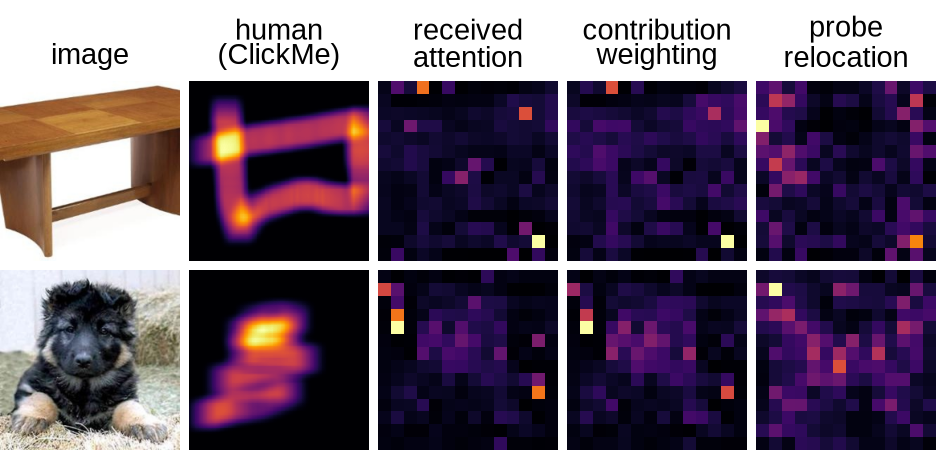
\includegraphics[width=4.7in]{example_maps}
\captionof{figure}{The first two fixed-seed examples, DeiT-S, layers 9--12. Colours show scores min--max normalised within each map; amplitudes are not comparable across panels. These images were not selected for correction gain.}
\label{fig:app-gallery-first}
\end{minipage}\end{center}

\begin{center}\begin{minipage}{\linewidth}
\centering
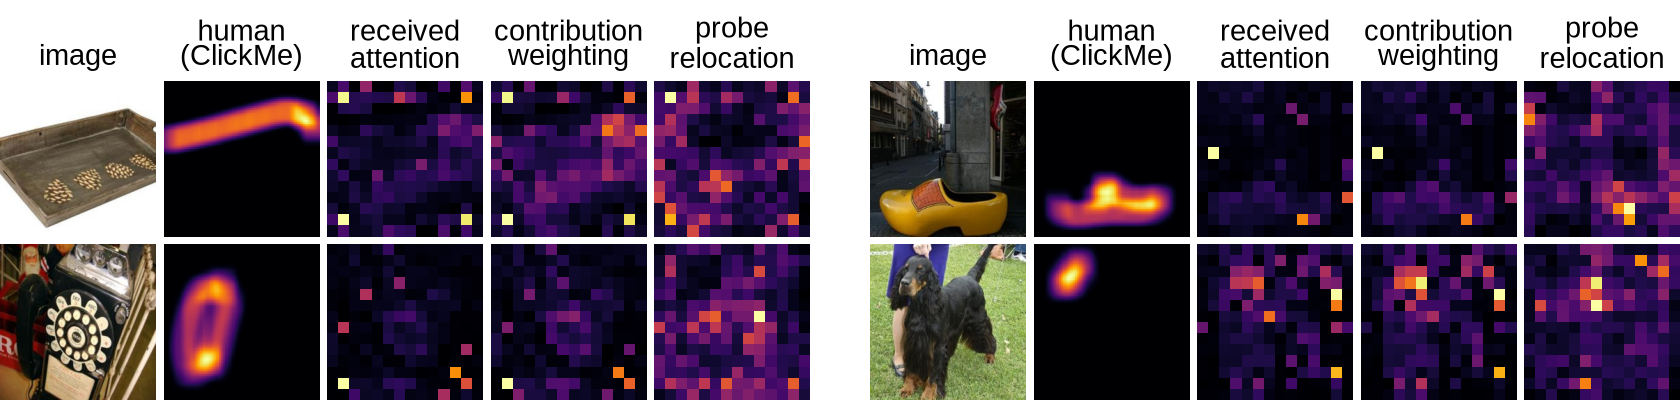
\includegraphics[width=5.5in]{example_maps_more}
\captionof{figure}{DeiT-S on four further ClickMe images, layers 9--12; colours are normalised within each map and do not compare amplitudes across panels.}
\label{fig:app-gallery}
\end{minipage}\end{center}

% =====================================================================================================
\clearpage
\section{Key parts of the code}
\label{app:code}

Given the attention $a_{ij}^h$ and values $v_j^h$ of a layer, the readings are:

\begin{lstlisting}[language=Python]
def received_and_contribution(p, v, w_o, prefix=1):
    # p: [B,H,T,T]; v: [B,H,T,d]; w_o: [D,H,d]
    # T includes CLS; values include the value-projection bias.
    gram = torch.einsum('dhe,dhf->hef', w_o, w_o)
    length = torch.einsum('bhne,hef,bhnf->bhn', v, gram, v)
    length = length.clamp_min(0).sqrt()
    received = p.sum(2)  # sum over queries
    s = received.sum(1)[:, prefix:]
    c = (received * length).sum(1)[:, prefix:]
    return s, c

def relocate(s, probs):  # source j to predicted position p
    return torch.einsum('bj,bjp->bp', s, probs)
\end{lstlisting}
